\documentclass[a4paper, 12pt]{article}
\usepackage{geometry} % Set margins
\geometry{margin=0.5in}

\usepackage{xcolor, graphicx, amsmath, amssymb, booktabs, longtable, hyperref}
\usepackage{lmodern} % Modern font
\usepackage{microtype} % Improves typography
\usepackage{caption} % Better control over captions
\usepackage{url} % Handle URLs
\usepackage{fancyhdr} % For headers and footers
\usepackage{setspace} % Line spacing
\usepackage{titlesec} % Section formatting
\usepackage{enumitem} % Custom list formatting
\usepackage{bookmark} % Better PDF navigation

\hypersetup{
    colorlinks=true,
    linkcolor=blue,
    citecolor=blue,
    urlcolor=blue,
    pdftitle={mBSW Model Data for the Rheology Textbook}
}

\title{\textbf{mBSW Model Data for the Rheology Textbook}}
\author{Atharva Modi \\ \texttt{asm18[at]illinois.edu}}
\date{\textit{Created: January 31, 2025}}

\begin{document}

\maketitle

\section*{Introduction}

This Jupyter Notebook (\texttt{mBSW\_data\_generation.ipynb}) computes
the relaxation modulus and dynamic moduli from a given set of mBSW
parameters and saves it to \texttt{.csv} files in the
\texttt{output\_data/} folder.

\section*{Summary}

\begin{itemize}

\item Data used here from the Hatzikiriakos et al.~(2000) is for
``PB-linear'', a well-entangled linear 1,4 polybutadiene:
\begin{quote}
\textit{Hatzikiriakos, S., Kapnistos, M., Vlassopoulos, D. et al. Relaxation time spectra of star polymers. Rheol. Acta 39, 38–43 (2000). https://doi.org/10.1007/s003970050005}
\end{quote}
\item The inferred parameters from the paper corresponding to our standard
mBSW form are:

\[
H(\tau) = e^{-\left(\frac{\tau}{\tau_{\max}}\right)^\beta} 
\left[ H_e \left( \frac{\tau}{\tau_{\max}} \right)^{n_e} + 
H_g \left( \frac{\tau}{\tau_e} \right)^{-n_g} \right]
\]

\begin{table}[htbp]
    \centering
    \begin{tabular}{ll}
        \toprule
        \textbf{Variable} & \textbf{Value} \\
        \midrule
        \(H_g\) (Pa)  & \(4.9 \times 10^5\) \\
        \(n_g\)       & \(0.67\) \\
        \(\tau_e\) (s) & \(0.86\) \\
        \(H_e\) (Pa)  & \(1.86 \times 10^5\) \\
        \(n_e\)       & \(0.30\) \\
        \(\tau_{\max}\) (s) & \(9.0 \times 10^5\) \\
        \(\beta\)     & \(2.0\) \\
        \bottomrule
    \end{tabular}
    \label{tab:parameters}
\end{table}

\item A free parameter not mentioned is the minimum cutoff relaxation time
\((\tau_{\text{min}})\). We used it to match the glassy modulus,
giving us:

\begin{itemize}
  \item \(\tau_{\text{min}} = 1.8\times 10^{-5}~\text{s}\)
  \item Calculated rubbery modulus, \(G_{\text{rubbery}} = 1.42~\text{MPa}\)
\end{itemize}

Additional analysis performed for improved model fitting and
uncertainty quantification. Details in \texttt{additional\_analysis/}.

\begin{figure}[htbp]
    \centering
    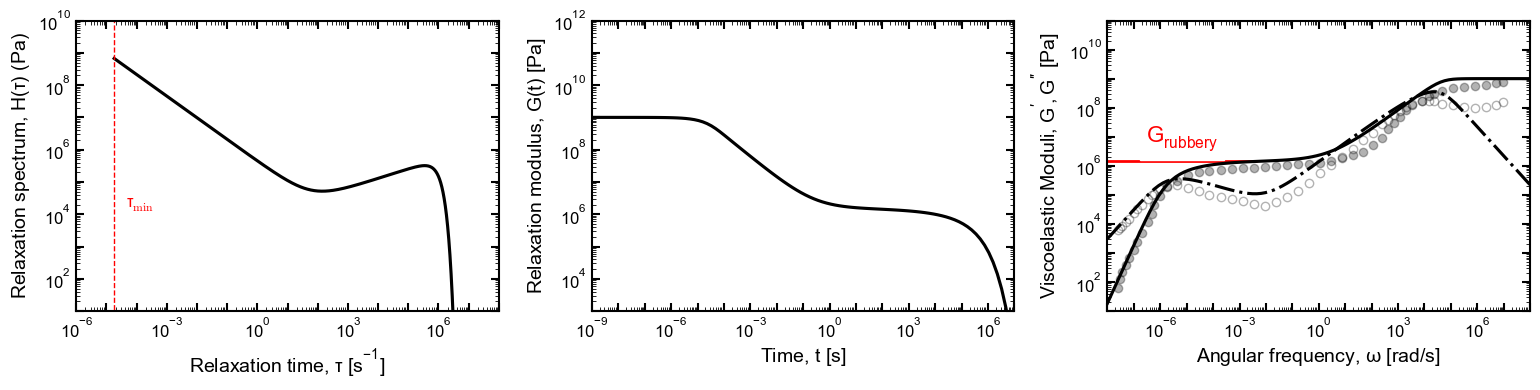
\includegraphics[width=0.99\linewidth]{model_data_figure.png}
    \label{fig:model_data}
\end{figure}
\end{itemize}

\section*{Contributing}

Feel free to modify the notebook for different datasets or additional
processing steps. Please contact asm{[}eighteen{]}{[}at{]}illinois.edu
for any feedback.

\section*{License}

This project is open-source and licensed under the MIT License.

\end{document}
